\documentclass{article}
\usepackage{bigstrut}
\usepackage{adjustbox}
\usepackage{graphicx}^^M
\usepackage[T1]{fontenc}
\usepackage{float}
\usepackage{gensymb}
\usepackage{siunitx}
\usepackage{subfig}

\usepackage[english]{babel}
\usepackage[utf8]{inputenc}
\usepackage{indentfirst}

\addtolength{\oddsidemargin}{-.875in}
\addtolength{\evensidemargin}{-.875in}
\addtolength{\textwidth}{1.75in}
\addtolength{\textheight}{1in}

\begin{document}
\title{Modeling and Simulation Report}
\begin{titlepage}
    \centering
	{\scshape\LARGE Optimization of Average Waiting Time at Bus Stops \par}
	\vspace{.5cm}
    {\scshape By:\par}
	{\scshape Steven Nichols, Akshay Sampath, Marcin Wisniowski, \\
    Eric Kim, and Erika Suttmeier\par}
	\vfill
	{\scshape Modeling and Simulation, Final Project\par}
	\vspace{.5cm}
	{\scshape Stevens Institute of Technology\\CPE-345\par}
	\vspace{.5cm}
	{\scshape supervised by\\ Dr. Cristina Comaniciu\par}
    \vfill
% Bottom of the page
	{\scshape“I pledge my honor that I have abided by the Stevens Honor System.”\par}
	\vspace{.5cm}
	{\scshape Steven Nichols \hfill Date: 05/14/18\\Akshay Sampath \hfill Date: 05/14/18\\Marcin Wisniowski \hfill Date: 05/14/18\\ Eric Kim \hfill Date: 05/14/18\\ Erika Suttmeier \hfill Date: 05/14/18\\}
	\vspace{3cm}
\end{titlepage}

%-----ADDING FIGURES------
%\begin{figure}[h]
%\begin{center}
%\includegraphics[width=\textwidth]{IMAGE_NAME_HERE}
%\caption{CAPTION_HERE}
%\end{center}
%\end{figure}

%-----ADDING TABLES-------
%\begin{table}[h]
%\begin{center}
%\begin{tabular}{c|c|c|c|c}
%& Butterworth & Chebyshev & Linkwitz-Riley & Bessel\\
%\hline
%Passband Accuracy & 10 & 4 & 6 & 9\\
%\hline
%Filter Slope & 7 & 10 & 5 & 6\\
%\hline
%Impulse Response & 5 & 7 & 10 & 3\\
%\hline
%Popularity in Crossover Filters & 3 & 3 & 7 & 3\\
%\hline
%Total & 25 & 24 & 28 & 21\\
%\hline
%Rank & 2 & 3 & 1 & 4\\
%\end{tabular}
%\caption{ADD CAPTION HERE}
%\end{center}
%\end{table}

%-----ADDING IMAGES-----
%\begin{center}
%\includegraphics[width=400px]{Image_NAME_HERE}
%\end{center}

\tableofcontents
\newpage

\section{Project Objective}
\subsection{System Analysis}
For this project, the team decided to analyze and model a bus queuing system. Waiting is the least satisfying part of using public transportation, decreasing its satisfaction rates. While many people are willing to use public transportation to solve issues with getting to and from work, public transportation could become more widely used if bus terminal systems could be optimized for waiting times. 

Since bus systems vary in complexity, it was decided it would be best to model a simple bus system operating during peak hours. The queue length of the model is influenced by how often buses and passengers arrive. The team defined passenger arrivals to follow a Poisson process. The project’s performance metric is the average wait time in queue for the bus riders. The major objective of this simulation is to test various processes for the bus service time, determining the optimal way to design the bus transportation system. 

\subsection{Literature Review}
A significant amount of research was done to understand the current state of transportation studies and best apply empirical data. Salek and Machemehl’s “Characterizing Bus Transit Passenger Wait Times” (1999) served as a valuable resource, especially for realistic passenger inter-arrival times and services times to build our model. Salek and Machemehl studied how bus transit properties affect average waiting time at bus stations throughout Austin, Texas. This study was conducted through direct observation and video recordings throughout the year of 1998, and found that bus arrival time, which they refer to as Bus Line Headway, as the largest predictor of average user wait time. "The experimental data were collected in a six-month period at several bus transfer centers and bus stations in the city of Austin, Texas" [1].

\subsection{Hypothesis}
As is conventional wisdom in the transportation studies field, average wait time is minimized when bus arrival time is perfectly deterministic. We hope to confirm this hypothesis with our model, and in systems where deterministic bus schedules are not possible, find which random systems are optimal for minimizing average wait time in queue.


\section{Mathematical Model}
   In order to correctly model the bus system, the group explored the distribution times and service times on one bus, hoping to expand these values to further research cases in the future.Through a reading of “Characterizing Bus Transit Passenger Wait Times” (1999), we were able to obtain references for certain parameters in our simulation to make sure it reflected the real-world conditions under which transportation systems operate. 
  
For the scope of our model, the two most important metrics in the table below are BLH (Bus Line Headway) and WAIT (Total Passenger Wait Time). BLH, as mentioned previously, is time between bus arrivals based on observational data, and WAIT is the observed average wait time of passengers. Mean BLH was used as a baseline service time to select a realistic range of service times to be simulated in our model. Deterministic distributions of 5, 10, 15, and 20 minutes were tested as well as Gaussian distributions with the following parameters: mean of 10 and standard deviation of 5, mean of 10 and standard deviation of 1, and mean of 5 and standard deviation of 5. The mean WAIT served as a benchmark for Average Queue Wait Time in our model, but deviates from our model data significantly for a number of reasons, which we will explore in more detail in the Verification/Validation section. 

   
   \newpage
   \begin{figure}[h]
	\begin{center}
	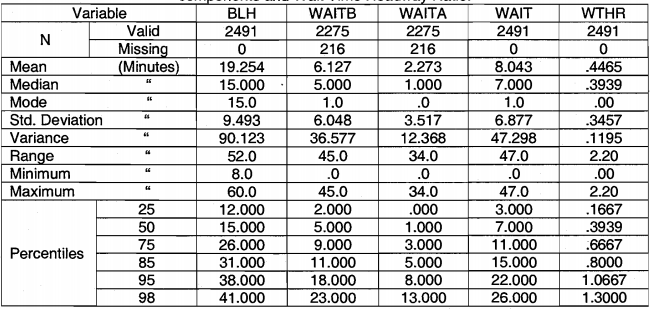
\includegraphics[width=400px]{Paper_Data_Table_1.png}
	\caption{Descriptive Statistics of the System Examined by Salek and Machemehl}
	\end{center}
	\end{figure}
    
\subsection{Inter-arrival Times}
   The model starts with "Source Once" which fills all of the bus seats in order to mimic a completely filled bus rolling up to a station. The group looked to follow a rush hour type of system in order to run the model through the largest queues of the bus's lifetime and optimize based on that fact. Afterwards, the normal source takes over and makes the commuters arrive at the bus terminal with an exponential distribution of inter-arrival times. 
 
\subsection{Departure Events}
   In order to correctly model a bus system within Omnet++[3], the event-based system runs during the modeled times that the bus arrives at the terminal. At this time, some seats on the bus empty as people leave the bus, while others fill to mimic new commuters entering to get to their locations. Meanwhile, between the entrance and exit of commuters onto and off the bus, the queue grows between the terminal times.
   
   The bus server itself is split into twenty one different bus seats which act as servers in the case of this model. Each bus seat is described to be either filled, or empty and accepting new arrivals. Each of the seats act as ideal copies of each other, and they are interchangeable to the commuters that arrive on the bus. Furthermore, some commuters stay on their seats through multiple departure events. This does not mean that a commuter will stay on the bus for one full cycle but instead indicates that the seat that they are occupying will be filled when the bus returns to the station. 

\subsection{Statistics Sink}
	The sink at the end is used to store statistical data for the user to explore when making inferences on improvements. During the simulation, multiple different bus server departure times were used to try and explore to find the most optimal bus service times. The departure distributions were explored to be either deterministic (as many are in the real world in order to simplify times tables for bus arrival times) as well as a truncated normal (to best estimate near an average amount of travel time between two stops with added variance). 
    
    \vspace{1cm}
    Below is the system model explained above in a tabular form. 
 	\begin{figure}[h]
	\begin{center}
	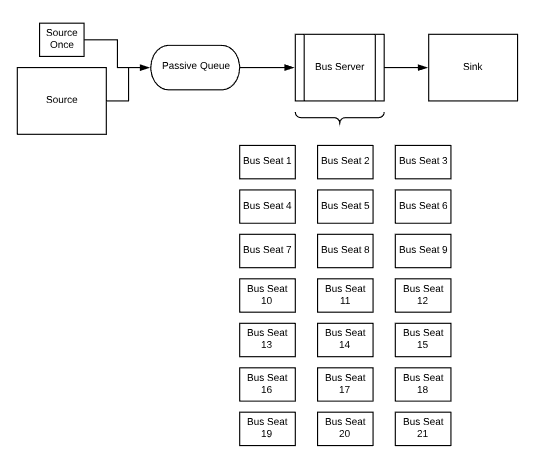
\includegraphics[width=400px]{Model_Graphic_v2.png}
	\caption{Expanded System Model of One Bus Server}
	\end{center}
	\end{figure}
  
  Our model used the following initialization data all gathered from online reference sources:

  	\begin{figure}[h]
	\begin{center}
	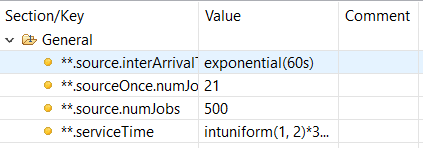
\includegraphics[width=150px]{ini_file.png}
	\caption{Initialization Parameters}
	\end{center}
	\end{figure}

\section{Snapshot of simulation}
	After obtaining all necessary data values, the model was constructed within Omnet++ in order to model the bus times. Similarly, the rough construction of the system model above was used in order create the model within Omnet++. After multiple different iterations, the model below was finalized. Within Omnet++[3], the source and source once was used in order to act as the arrival commuters for the system, while the servers were used to act as the bus seats within the system. The passive queue also grew as the time ticked on.
    
	\begin{figure}[h]
	\begin{center}
    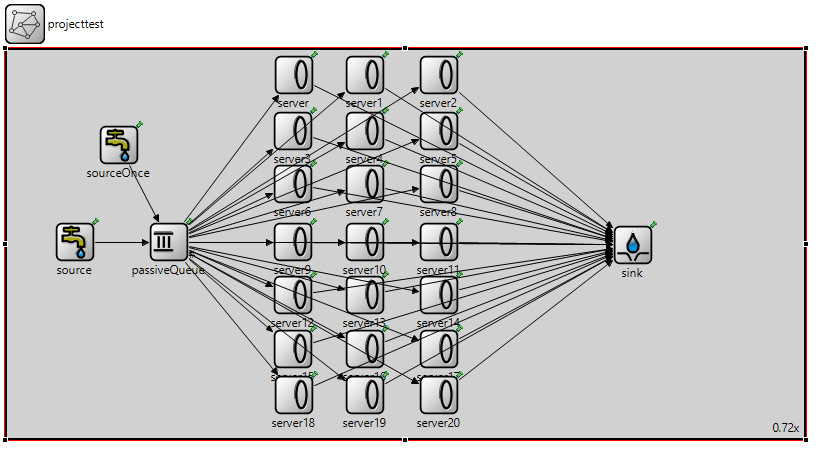
\includegraphics[width=300px]{Omnet++_System_Model.png}
    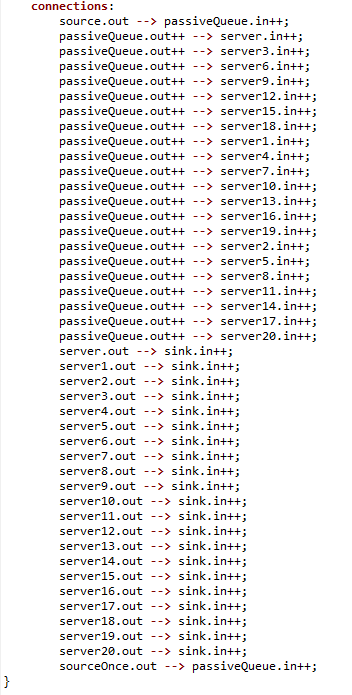
\includegraphics[width=150px]{Model_Connections.png}
	\caption{Omnet++ Simulation}
	\end{center}
	\end{figure} 
	
\section{Simulation Results}
	After building the simulation, the model was run using a core 500 commuters across all the different simulations. In order to gain insight from the model, the distribution of the departure times from the seats was changed from a Deterministic distribution of times for the arrival of buses to a truncated normal time of bus arrivals. Below are tables of the results of each of the tests.
    \vspace{1cm}
    \begin{table}[h]
	\begin{center}
	\begin{tabular}{c|c|c|c|c}
	& Deterministic(5) & Deterministic(10) & Deterministic(15) & Deterministic(20) \\
	\hline
	Average Queue Wait Time (min) & 2.7742 & 3.093 & 28.3517 & 130.525\\
	\hline	
	Average Queue Length & 0.02715 & 0.42684 & 24.57160 & 85.87214\\
	\hline	
	\end{tabular}
	\caption{Deterministic Distribution Results}
	\end{center}
	\end{table}
    
    \begin{table}[h]
	\begin{center}
	\begin{tabular}{c|c|c|c}
	& TruncNorm(5,5) & TruncNorm(10,1) & TruncNorm(10,5) \\
	\hline
	Average Queue Wait Time (min) & 0.365 & 3.985 & 2.2688\\
	\hline	
	Average Queue Length & 0.00499 & 1.48891 & 0.80558\\
	\hline	
	\end{tabular}
	\caption{Truncated Normal Time Distribution Results}
	\end{center}
	\end{table}
   
   \newpage
\subsection{Analysis}
The purpose of testing the two different types of distributions was to determine which service distribution model resulted in the lowest average queue waiting time for bus passengers. Overall, the deterministic distribution had the longest average queue waiting times and queue lengths compared to those of the truncated normal times of bus arrivals. Decreasing the distribution times significantly reduced the average queue wait time and queue length. For the truncated normal distribution, both the average queue wait time and queue length were more sensitive to the mean values than the standard deviation values. The truncated normal distribution with the mean of 5 and standard deviation of 5 had the lowest overall average queue wait time and queue length. 

The normally distributed arrival times, with the exception of the 10 minute mean and 1 minute standard deviation trial, were with a wildly irregular system, and would not be reasonable to recommend for implementation in a physical system. Of the constant time models, both the 5 minute and 10 minute arrival times of the bus yielded similar, and acceptably low, average wait times. As they both would be acceptable for use, in practical applications, the 10 minute constant arrival time of the bus would be the most cost effective solution to moving this volume of people with this size bus.

\section{Verification/Validation}
This study has attempted to develop a simulation in order to evaluate the best passenger wait time for an arriving bus. The model that was created by the team analysed the effect that altering distribution times had on the average wait time for a bus as well as the average length of a queue. The model results, for both models, show that passenger wait time and passenger queue length both were strongly influenced by the different bus distributions. The team noticed that the generated results mostly followed their expectations. They hypothesized that the best distribution times for the deterministic model would be between the 10-15 minute periods, and the data shows that the team was on the right track. 

The team’s ideal system was a deterministic system design. However, during the simulations the team noticed that the Gaussian service times had better metrics. This performance shows that during difficult traffic conditions bus transportation systems can adapt to unpredictable schedules by sending more buses into the system.

Moreover, the average waiting time in our simulation was found to be significantly less than our reference model. This difference is to be expected, as our model failed to take in to account many different factors, mainly human behavior. The reference model was based on observational data, which took note of the effects human actions and decisions played into the inter-arrival times of the passengers. The Poisson inter-arrival time we used in the model was much more regular than it would be in real life and thus easier for a simulated system to handle. 



\section{References}
\begin{enumerate}
\item Salek, Machemehel. "Characterizing Bus Transit Passenger Wait Times", Final Research Report 167211-1, Conducted for Southwest Region University Transportation Center, 1999.
\item Hughes-Cromwick, "2017 Public Transportation Fact Book", 68th Edition, Conducted for the American Public Transportation Association, 2017.
\item Varga, Andras. “Chapters.” OMNeT++ Discrete Event Simulator - Home, www.omnetpp.org/doc/omnetpp/manual/.
\item Comaniciu, Cristina. “Modeling and Simulation.” CPE 345 Lectures. CPE 345 Lectures, Hoboken, NJ, 07030.
\end{enumerate}




\end{document}